\documentclass[simplex.tex]{subfiles}
% NO NEED TO INPUT PREAMBLES HERE
% packages are inherited; you can compile this on its own
\begin{document}
\subsection{knor: K-means NUMA Optimized Routines}

%% Jan

The \textsf{knor} library is a set of tools enabling users to perform the
popular k-means algorithm at scale at speeds of 10x-100x time of that of popular
frameworks in use today like Spark's MLlib, H$^2$O and GraphLab(Turi, Dato).
We provide highly optimized routines for the
following cases:

\begin{compactitem}
    \item Big-data that fits into the main memory (RAM) of a single machine, use
        \textsf{knori}. \newline
    \item Big-data that fits into the aggregate main memory (RAM) of a cluster
        of distributed machines in the cloud, use \textsf{knord}. \newline
    \item Big-data that cannot fit into the main memory (RAM) of a single machine,
        but can be placed out-of-corek, on disk, use \textsf{knors}.
\end{compactitem}

As part of efforts to make \textsf{knor} as user-friendly as possible we now
support it on any platform via Docker containerization. We provide a one line
installation procedure found at The repo's
\href{https://github.com/disa-mhembere/knor/}{landing page}.
We further provide detailed instructions on how to use and extract data within
the \textsf{knor} framework.\\


We recently submitted the \textsf{knor} paper to High-Performance Parallel and
Distributed Computing (HPDC 2017) and publicly released it to
\href{https://arxiv.org/abs/1606.08905}{arxiv}.

Figure \ref{fig:rmvm} compares the performance of our in-memory (\textsf{knori})
and our semi-external memory (\textsf{knors}) routines to our competitors.
Distributed results (\textsf{knord}) can be found within the paper.\\


%% >> March 
We previously described the \textsf{knor} library. As a set of tools enabling
users to perform the popular k-means algorithm at scale at speeds of 10x-100x
time of that of popular frameworks in use today like Spark's MLlib, H$^2$O
and GraphLab(Turi, Dato). \\

We would like to report that our \textsf{knor} paper that was submitted
to the ACM Symposium on High-Performance Parallel and Distributed Computing (HPDC 2017)
and publicly released it to \href{https://arxiv.org/abs/1606.08905}{arxiv}
was \textbf{accepted} for publication to the 26th proceedings of HPDC.

%% << MARCH

\begin{figure}[!h]
\begin{cframed}
\centering
%\begin{figure}[!htb]
    \footnotesize
    %\vspace{-25pt}
    \begin{subfigure}{1\textwidth}
    \centering
    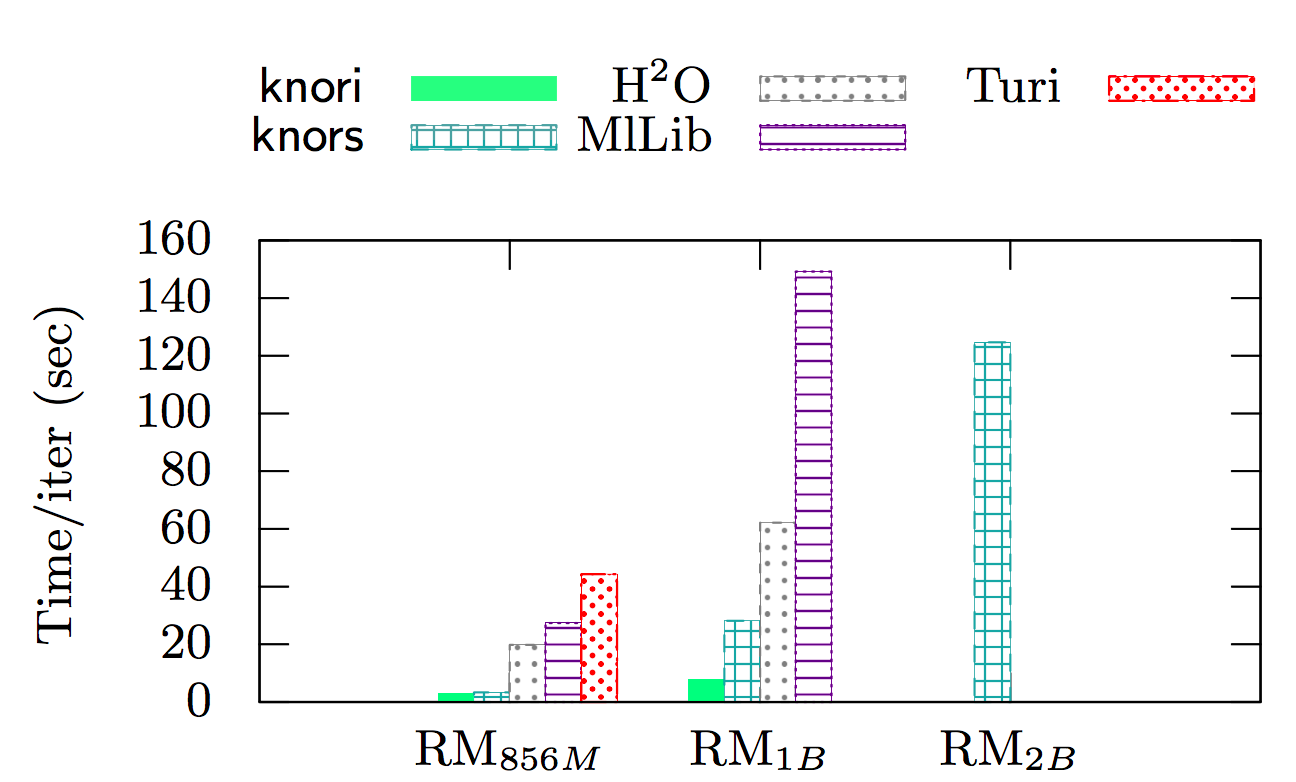
\includegraphics[width=0.9\textwidth]{../../figs/perf.iter.rmvm.png}
    \caption{Per iteration time elapsed of each routine.}
    \label{fig:perf-rmvm}
    \end{subfigure}

    \begin{subfigure}{1\textwidth}
    \centering
    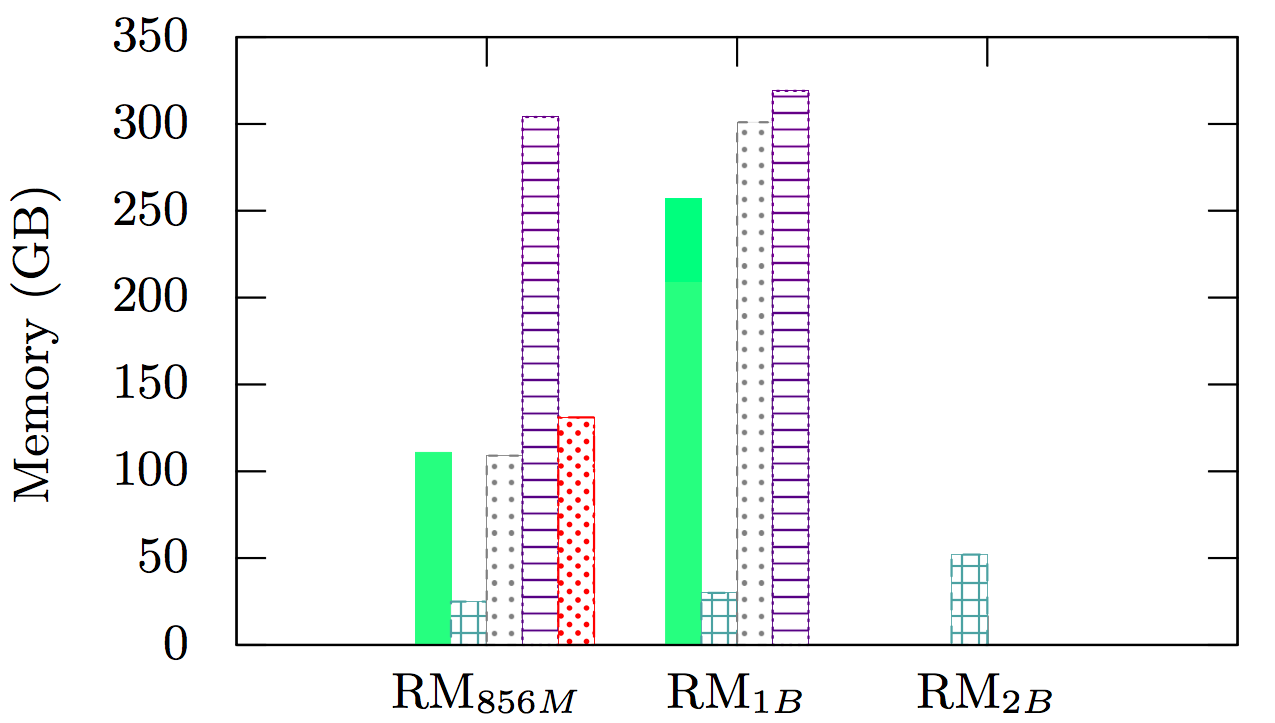
\includegraphics[width=0.9\textwidth]{../../figs/mem.rmvm.png}
    \caption{Memory consumption of each routine.}
    \label{fig:mem-rmvm}
    \end{subfigure}
    \caption{Speed and Memory comparison on randomly generated datasets
        (i) RM$_{856M}$, a 856 Million X 16 dataset of size 103GB and
        (ii) RM$_{1B}$, a 1 Billion X 32 dataset of size 251 GB and (iii) RM$_{2B}$,
        a 2 Billion X 64 dataset of size 1.1 TB. Turi is unable to run on RM$_{1B}$
        on our machine and only SEM routines are able to run on RU$_{2B}$ on our
    machine with 48 Cores and 1 TB of RAM.}
    \label{fig:rmvm}
\end{cframed}
\end{figure}
\clearpage

%% Feb



\end{document}
